\documentclass[12pt]{SeminarskiADS}

\begin{document}
\Predmet{Adaptivni diskretni sistemi i neuralne mreže}
\Nastavnik{Prof. dr Miloš Daković}
\Naslov{Obrada EKG signala pomoću LMS algoritma i klasifikacija pomoću SVM klasifikatora}
\Kandidat{Andrej Jokić}
\Indeks{19/2018}
\Datum{januar 2019.}
\maketitle 


\section{Uvod}
Elektrokardiografija je veoma značajna u dijagnozi mnogih srčanih poremećaja. Elektrokardiogram (EKG) je grafički prikaz električne aktivnosti srca. Na njemu su prikazane promjene bioelektričnog potencijala u vremenu. Mnogi poremećaji u radu srca se mogu uočiti analizom oblika EKG signala i varijacije pulsa (\emph{HRV - Heart Rate Variation}) \cite{gl}. 

Jedan od široko rasprostranjenih srčanih poremećaja je aritmija (poremećaj srčanog ritma). Aritmija obuhvata više srčanih bolesti kod kojih su otkucaji srca nepravilni, prespori ili pak prebrzi \cite{what_is_arr}. Ovakvi poremećaji se dosta pouzdano mogu otkriti analizom EKG snimka. Kako biosignali nisu stacionarni, indikacije ovog poremećaja se mogu pojaviti u nasumičnim trenucima. Naime, simptomi aritmije često nisu prisutni sve vrijeme, već se pojavljuju u nepravilnim intervalima u toku dana. Stoga, radi efektivne dijagnoze, EKG se ponekad snima i po nekoliko sati. Analiza ovako velike količine podataka je teška i oduzima mnogo vremena. Takođe, postoji mogućnost da ljekar ne uoči ili pogrešno protumači neki značajan podatak. Zbog toga se dosta radi na razvoju računarskih tehnika za analizu EKG snimaka \cite{ecg_multiclass_svm}.

U toku snimanja i prenosa, EKG signali često bivaju zahvaćeni određenom količinom šuma. Prisustvo šuma može otežati analizu ili prouzrokovati pogrešno tumačenje podataka. Zato je prije analize potrebno filtrirati signal kako bi se uklonilo što više šuma. Neke od tehnika filtriranja koje se koriste za EKG signal su IIR notch filtri, FIR filtri, adaptivni filtri, Wavelet transformacija itd. \cite{ecg_denoise} U ovom radu ćemo primijeniti adaptivni filtar zasnovan na LMS algoritmu. 

Kako bi se signali efektivno klasifikovali, potrebno je izdvojiti karakteristične parametre iz EKG signala. SVM klasifikator će na osnovu ovih parametara svrstati signale u odgovarajuće klase. EKG signali sadrže značajne podatke i u vremenskom i u frekvencijskom domenu. Zato se za izdvajanje parametara EKG signala često koristi diskretna wavelet transformacija. DWT omogućava da se ogromna količina podataka koja karakteriše EKG signal komprimuje u mali broj značajnih parametara. 


%Nesto da se u poslednjim godinama mnogo posvecuje paznja razvoju tehnika masinskog ucenja za 
Mašinsko učenje omogućava računaru da analizom velike količine podataka ``uoči'' veze između pojedinih elemenata. Mnogi naučni radovi istražuju primjenu različitih algoritama mašinskog učenja u klasifikaciji EKG signala. Neke od tehnika koje se primjenjuju su KNN (\emph{K-Nearest-Neighbor}), \emph{Neuro Fuzzy} klasifikator, SVM (\emph{Support Vector Machine}), \emph{Deep Learning} itd. Rezultati su pokazali da najbolje performanse i najveću tačnost klasifikacije EKG signala ima SVM klasifikator. 

%Visokofrekventni šumovi kod EKG signala najčešće obuhvataju bijeli gausov šum i sinusoidalne smetnje iz električne mreže. 

\section{EKG}

Za dobro funkcionisanje kardiovaskularnog sistema, neophodno je da se srčani mišići kontrahuju u pravilnom ritmu. Ritam kontrakcija srčanog mišića kontrolišu električni impulsi koji potiču iz \emph{sinusnog čvora} (\emph{P ćelije}). Dio struja prouzrokovanih električnim impulsima stiže do površine kože, gdje izazivaju promjene električnog potencijala. Elektrokardiograf je zapravo precizan galvanometar koji mjeri ove potencijale. Kod standardnog EKG-a, na tijelo pacijenta se postavlja 12 elektroda, koje mjere razlike potencijala između određenih tačaka na površini kože.

Na slici \ref{ecg_otkucaj} je prikazan jedan otkucaj srca na EKG snimku kod zdrave osobe (normalni sinusni ritam). Jedan otkucaj se sastoji iz P talasa, QRS kompleksa i T talasa. Za analizu varijacije pulsa (HRV) najznačajnija je detekcija QRS kompleksa, tj. detekcija R pika. Automatska detekcija R-pikova nije jednostavna, kako zbog fiziološke varijabilnosti QRS kompleksa, tako i zbog prisustva raznih šumova i smetnji u EKG signalu \cite{rpeak_dwt}. Postoje mnogi softverski paketi za detekciju R pikova i HRV analizu. U ovom radu je korišćen open-source toolbox za \emph{Matlab} softverski paket, ``Physionet Cardiovascular Signal Toolbox'' \cite{physionet_tbx}. Primjeri EKG signala su preuzeti iz opšteprihvaćene MIT-BIH baze. Uz same EKG signale, u ovoj bazi su dostupni i ručno obilježeni R-pikovi \cite{mit_bih}. %TODO dodaj koje signale si preuzeo i koliko njih, dužina, Fs...




%sto je ekg

%qrs

%slika qrs

\begin{figure}[h]
\centering
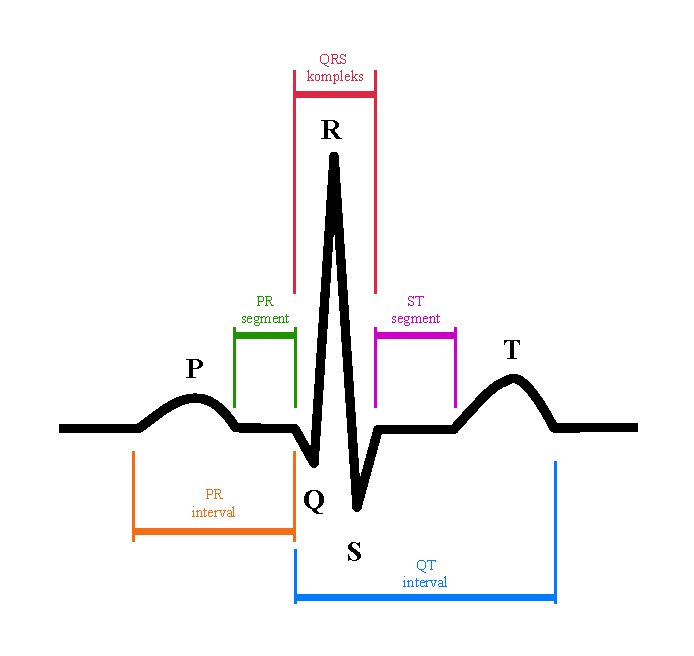
\includegraphics[width=0.8\textwidth]{ecg_otkucaj}
\caption{Jedan otkucaj srca na EKG snimku}
\label{ecg_otkucaj}
\end{figure}


\section{LMS filtriranje}
\label{sec:lms}

EKG signali često sadrže određenu količinu šuma koji nastaje u toku snimanja ili prenosa signala. Uglavnom su zastupljene dvije vrste šuma. Visokofrekventni šumovi obuhvataju šum \emph{elektromiograma} (uređaj kojim se snimaju bioelektrični potencijali), bijeli gausov šum i sinusoidalne smetnje iz električne mreže (50/60Hz). Niskofrekventni šum koji je prisutan kod EKG signala naziva se \emph{baseline wander}. Ovaj šum nastaje kao posljedica fizičkog pomjeranja i disanja pacijenta. Takođe, ako se EKG signal prenosi bežičnom vezom, prisutan je i kanalni šum. Ovaj šum takođe ima karakteristike bijelog Gausovog šuma. 

Prisustvo veće količine šuma značajno utiče na oblik EKG signala. Ovo može izazvati pogrešno tumačenje podataka i grešku u klasifikaciji. Prema tome, potrebno je izvršiti obradu signala kako bi se uklonila što veća količina šuma prije izdvajanja parametara i klasifikacije. Usljed promjenljive prirode EKG signala, uklanjanje šuma iz EKG signala nije jednostavno. Neke od tehnika koje se koriste su IIR notch filtri (za uklanjanje sinusoidalnih smetnji), \emph{Wavelet Transform Thresholding}, \emph{Bionic Wavelet Transform}, adaptivni filtri. Adaptivno filtriranje podrazumijeva upotrebu LMS, RLS ili EMD (\emph{Empirical Mode Decomposition}) algoritama. Tehnike zasnovane na wavelet transformaciji, RLS i EMD su računski veoma zahtjevne. U ovom radu će biti primijenjeno filtriranje pomoću LMS algoritma.

LMS algoritam je veoma efikasan u odnosu na ostale adaptivne metode filtriranja. U prenosnim medicninskim uređajima primjena ovog algoritma omogućava upotrebu jednostavnijeg hardvera i manju potrošnju električne energije. Takođe, ovaj algoritam ima dobre performanse uklanjanja šuma kod vremenski promjenljivih signala.

\begin{figure}[tbp]
\centering
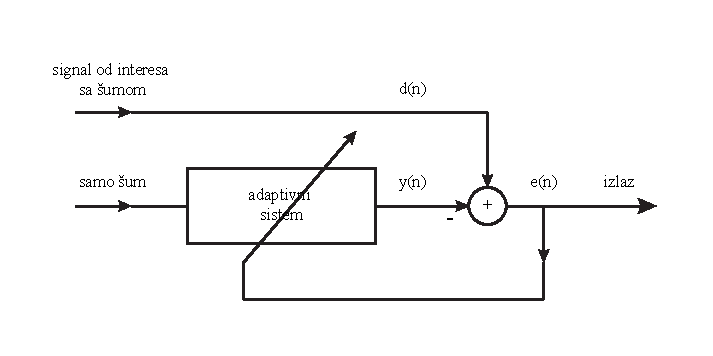
\includegraphics[width=0.9\textwidth]{lms_denoise}
\caption{Adaptivni sistem za uklanjanje šuma}
\label{lms_denoise}
\end{figure}

\section{Izdvajanje parametara}
\label{sec:extraction}
%TODO jos prije ovoga
Nakon određivanja R-pikova, na osnovu RR intervala se vrši HRV analiza. Kao rezultat ove analize dobijaju se određeni parametri EKG signala, na osnovu kojih se može izvršiti klasifikacija, tj. dijagnoza srčanog poremećaja. HRV parametri se mogu podijeliti na parametre u vremenskom i parametre u frekvencijskom domenu:

\begin{itemize}
\item \textbf{Parametri u vremenskom domenu: } NN mean, NN mode, NN median, NN skew, NN kurtosis, NNiqr, SDNN, RMSSD, pNN50
\item \textbf{Parametri u frekvencijskom domenu: } ULF snaga, VLF snaga, LF snaga, HF snaga, LF/HF odnos, totalna spektralna snaga
\end{itemize}
%prvo napisem koji sumovi zahvataju signal, kako uticu na filtriranje

%onda primjenu LMS algoritma za uklanjanje suma

%slika lms denoising i denlms

%NLMS i DENLMS

%prikaz rezultata


\clearpage
\begin{thebibliography}{99}
\bibitem{gl} C. Venkatesan, P. Karthigaikumar, Anand Paul, S. Satheeskumaran, R. Kumar, ``ECG Signal Preprocessing and SVM Classifier Based Abnormality Detection in Remote Healthcare Applications'', IEEE Access, 2018.

\bibitem{what_is_arr} National Heart, Lung, and Blood Institute, ``What is arrhythmia?''
\url{https://www.nhlbi.nih.gov/health-topics/arrhythmia}

\bibitem{ecg_multiclass_svm} Elif Derya Übeyli, ``ECG beats classification using multiclass support vector machines with error correcting output codes'', Digital Signal Processing, 2007.

\bibitem{ecg_denoise} Aswathy Velayudhan, Soniya Peter, ``Noise Analysis and Different Denoising Techniques of ECG Signal - A Survey'', IOSR-JECE, 2016.

\bibitem{dsp} Ljubiša Stanković, ``Digital Signal Processing''

\bibitem{rpeak_dwt} K. Deergha Rao, ``DWT Based Detection of R-peaks and Data Compression of ECG Signals'', IETE Journal of Research, 1997.

\bibitem{physionet_tbx} Vest A, Da Poian G, Li Q, Liu C, Nemati S, Shah A, Clifford GD, ``An Open Source Benchmarked Toolbox for Cardiovascular Waveform and Interval Analysis'', Physiological Measurement (In Press), DOI:10.5281/zenodo.1243111, 2018.

\bibitem{mit_bih} Moody GB, Mark RG, ``The impact of the MIT-BIH Arrhythmia Database'', IEEE Eng in Med and Biol 20(3):45-50, May-June 2001 (PMID: 11446209). 


\end{thebibliography}


\end{document}
